\chapter{CodeDocumentation}
\label{apx:Code}

The code documentation aims to describe the overall structure of our implementation as well as the main functions of our PHP and JavaScript code. We first provide a general overview of the code structure, before going into more code specific details. 

\section{Structure}
\label{sec:CodeStructure}
When creating such a comprehensive web site it is very important to create a code and document structure that clearly separates the different modules. These modules were in our case; backend code, JavaScript code, style code, markup code and image files. The backend code written in PHP is divided into three categories; documents performing database queries, documents creating forms or pages that will be fetched using AJAX and lastly documents with general functions for images, sharing and login. The JavaScript code consists mostly of functions performed when a page is loaded or when the user interacts with a page. This can be through mouse events or text typed. The style code is a collection of CSS documents used to style the different HTML elements, such as divs, buttons and text fields. Lastly all image files are separated from the code documents and placed in its own folder. In figure \ref{fig:CodeStructureStruc} the overall structure can be viewed.

\begin{figure}[ht!]
  \centering
  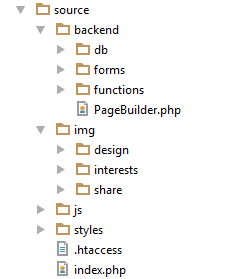
\includegraphics[width=50mm]{./Appendix/CodeDocumentation/img/structure}
  \caption{Overall structure of the code.}
  \label{fig:CodeStructureStruc}
\end{figure}

\section{Details}
\label{sec:CodeDetails}

\subsection{Backend/DB}
\label{subsec:CodeDetailsBackendDB}

\subsubsection{DBComments}
\begin{minipage}{\linewidth}
  \centering
  \setlength{\tabcolsep}{12pt}
  \rowcolors{1}{blue!20}{blue!10}
  \begin{tabular}{|p{0.35\linewidth}|p{0.55\linewidth}|}
  \hline
  \cellcolor{gray!25} Function & \cellcolor{gray!25} Description \\
  \hline
  getComments(threadID) & Fetching all comments related to a threadID from the database. \\
  insertComment(threadID, parent, username, comment) & Inserts a new comment into the database. All comments have a creator (username), a threadID and the comment itself. If the comment is a reply, it also has a parent comment. \\
  \hline  
  \end{tabular}
\end{minipage}

\subsubsection{DBEvents}
\begin{minipage}{\linewidth}
  \centering
  \setlength{\tabcolsep}{12pt}
  \rowcolors{1}{blue!20}{blue!10}
  \begin{tabular}{|p{0.35\linewidth}|p{0.55\linewidth}|}
  \hline
  \cellcolor{gray!25} Function & \cellcolor{gray!25} Description \\
  \hline
  addEvent(creator, title, description, interests, coordinates, numPeople, time) & Validates and inserts a new event into the database. All events have a creator(username), a string title and description, max number of people and time (unix timestamp). Additionally they are tagged with interests and geographical coordinates. \\
  fetchEvent(eventID) & Fetches an event based on the event ID. \\
  voteEvent(eventID, up, down) & Adds up number of positive votes and down number of negative votes to an event. \\
  searchEvents(interests, bounds, page) & Fetches a page of events matching tagged under interests within a geographical bound. \\
  \hline  
  \end{tabular}
\end{minipage}

\subsubsection{DBInterests}
\begin{minipage}{\linewidth}
  \centering
  \setlength{\tabcolsep}{12pt}
  \rowcolors{1}{blue!20}{blue!10}
  \begin{tabular}{|p{0.35\linewidth}|p{0.55\linewidth}|}
  \hline
  \cellcolor{gray!25} Function & \cellcolor{gray!25} Description \\
  \hline
  getInterest(id) & Fetches the interest with the given id. \\
  HTTP GET interest & Returns a JSON array of interests that begin with interest. \\
  \hline  
  \end{tabular}
\end{minipage}

\subsubsection{DBPhotos}
\begin{minipage}{\linewidth}
  \centering
  \setlength{\tabcolsep}{12pt}
  \rowcolors{1}{blue!20}{blue!10}
  \begin{tabular}{|p{0.35\linewidth}|p{0.55\linewidth}|}
  \hline
  \cellcolor{gray!25} Function & \cellcolor{gray!25} Description \\
  \hline
  addPhoto(uploader, title, coordinates, interests, description) & Validates and inserts a new photo into the database. All photos have an uploader, a string title and description. Additionally they are tagged with interests and geographical coordinates. \\
  removePhoto(id) & Removes a photo from the database based on the photo id. \\
  getPhotoDetails(id) & Fetches all data of a photo based on the photo id. \\
  votePhoto(id, up, down) & Adds up number of positive votes and down number of negative votes to an event. \\
  searchPhotos(interests, bounds, page) & Fetches a page of photos matching tagged interests within a geographical bound. \\
  \hline  
  \end{tabular}
\end{minipage}

\subsubsection{DBUsers}
\begin{minipage}{\linewidth}
  \centering
  \setlength{\tabcolsep}{12pt}
  \rowcolors{1}{blue!20}{blue!10}
  \begin{tabular}{|p{0.35\linewidth}|p{0.55\linewidth}|}
  \hline
  \cellcolor{gray!25} Function & \cellcolor{gray!25} Description \\
  \hline
  addUser(username, password, firstName, lastName, gender) & Validates and inserts a new user into the database. All users have a username and a password, as well as a first name, a last name and a gender. \\
  checkLogin(username, password) & Checks if the password matches the given username. \\
  usernameExists(username) & Returns true if a username is already taken. \\
  \hline  
  \end{tabular}
\end{minipage}

\subsubsection{DBVotes}
\begin{minipage}{\linewidth}
  \centering
  \setlength{\tabcolsep}{12pt}
  \rowcolors{1}{blue!20}{blue!10}
  \begin{tabular}{|p{0.35\linewidth}|p{0.55\linewidth}|}
  \hline
  \cellcolor{gray!25} Function & \cellcolor{gray!25} Description \\
  \hline
  registerVote(contentID, vote) & Registers that the logged in user has voted vote on contentID. \\
  didVote(contentID) & Returns whether the logged in user has voted on contentID. \\
  \hline  
  \end{tabular}
\end{minipage}

\subsection{Backend/Forms}
\label{subsec:CodeDetailsBackendForms}

\subsubsection{CommentForm}
\begin{minipage}{\linewidth}
  \centering
  \setlength{\tabcolsep}{12pt}
  \rowcolors{1}{blue!20}{blue!10}
  \begin{tabular}{|p{0.35\linewidth}|p{0.55\linewidth}|}
  \hline
  \cellcolor{gray!25} Function & \cellcolor{gray!25} Description \\
  \hline
  getCommentsForm(id) & Returns the full markup for the comment section for thread id. \\
  showComment(comments) & Creates the comment thread layout for current and all nested comments inside comments array. \\
  \hline
  \end{tabular}
\end{minipage}

\subsubsection{EventForm}
\begin{minipage}{\linewidth}
  \centering
  \setlength{\tabcolsep}{12pt}
  \rowcolors{1}{blue!20}{blue!10}
  \begin{tabular}{|p{0.35\linewidth}|p{0.55\linewidth}|}
  \hline
  \cellcolor{gray!25} Function & \cellcolor{gray!25} Description \\
  \hline
  HTTP POST & Passes on HTTP POST variables to DBEvent.addEvent(), returns JSON a formatted response. \\
  HTTP GET & Returns HTML for event creation form. \\
  \hline
  \end{tabular}
\end{minipage}

\subsubsection{GetLocation}
\begin{minipage}{\linewidth}
  \centering
  \setlength{\tabcolsep}{12pt}
  \rowcolors{1}{blue!20}{blue!10}
  \begin{tabular}{|p{0.35\linewidth}|p{0.55\linewidth}|}
  \hline
  \cellcolor{gray!25} Function & \cellcolor{gray!25} Description \\
  \hline
  HTTP POST image & Checks if image has EXIF GPS coordinates attached to it. \\
  \hline
  \end{tabular}
\end{minipage}

\subsubsection{LogForm}
\begin{minipage}{\linewidth}
  \centering
  \setlength{\tabcolsep}{12pt}
  \rowcolors{1}{blue!20}{blue!10}
  \begin{tabular}{|p{0.35\linewidth}|p{0.55\linewidth}|}
  \hline
  \cellcolor{gray!25} Function & \cellcolor{gray!25} Description \\
  \hline
  HTTP POST & Passes on HTTP POST variables to DBUsers.checkLogin(), returns JSON a formatted response. \\
  HTTP GET & Returns HTML for login form. \\
  \hline
  \end{tabular}
\end{minipage}

\subsubsection{MapLookup}
\begin{minipage}{\linewidth}
  \centering
  \setlength{\tabcolsep}{12pt}
  \rowcolors{1}{blue!20}{blue!10}
  \begin{tabular}{|p{0.35\linewidth}|p{0.55\linewidth}|}
  \hline
  \cellcolor{gray!25} Function & \cellcolor{gray!25} Description \\
  \hline
  HTTP GET & Creates a page with Google Maps location autocomplete and Google Maps map. Is meant to be opened in a separate window and used as a location selector: on window close, it returns the selected location. \\
  \hline
  \end{tabular}
\end{minipage}

\subsubsection{OverlayEvents}
\begin{minipage}{\linewidth}
  \centering
  \setlength{\tabcolsep}{12pt}
  \rowcolors{1}{blue!20}{blue!10}
  \begin{tabular}{|p{0.35\linewidth}|p{0.55\linewidth}|}
  \hline
  \cellcolor{gray!25} Function & \cellcolor{gray!25} Description \\
  \hline
  HTTP GET id & Returns HTML for the overlay with event details, comments and sharing for event id. \\
  \hline
  \end{tabular}
\end{minipage}

\subsubsection{OverlayPhotos}
\begin{minipage}{\linewidth}
  \centering
  \setlength{\tabcolsep}{12pt}
  \rowcolors{1}{blue!20}{blue!10}
  \begin{tabular}{|p{0.35\linewidth}|p{0.55\linewidth}|}
  \hline
  \cellcolor{gray!25} Function & \cellcolor{gray!25} Description \\
  \hline
  HTTP GET id & Returns HTML for the overlay with photo details, comments and sharing for photo id. \\
  \hline
  \end{tabular}
\end{minipage}

\subsubsection{RegForm}
\begin{minipage}{\linewidth}
  \centering
  \setlength{\tabcolsep}{12pt}
  \rowcolors{1}{blue!20}{blue!10}
  \begin{tabular}{|p{0.35\linewidth}|p{0.55\linewidth}|}
  \hline
  \cellcolor{gray!25} Function & \cellcolor{gray!25} Description \\
  \hline
  HTTP POST & Passes on HTTP POST variables to DBUsers.addUser(), returns JSON a formatted response. \\
  HTTP GET & Returns HTML for register form. \\
  \hline
  \end{tabular}
\end{minipage}

\subsubsection{UploadPhoto}
\begin{minipage}{\linewidth}
  \centering
  \setlength{\tabcolsep}{12pt}
  \rowcolors{1}{blue!20}{blue!10}
  \begin{tabular}{|p{0.35\linewidth}|p{0.55\linewidth}|}
  \hline
  \cellcolor{gray!25} Function & \cellcolor{gray!25} Description \\
  \hline
  uploadImage(title, interests, description, image, coordinates) & Validates and scales an image before inserting it into the database via DBPhotos.addPhoto(). \\
  HTTP GET & Returns HTML for upload image form. \\
  HTTP POST & Passes on HTTP POST variables to uploadImage(), returns JSON a formatted response. \\
  \hline
  \end{tabular}
\end{minipage}

\subsubsection{VoteForm}
\begin{minipage}{\linewidth}
  \centering
  \setlength{\tabcolsep}{12pt}
  \rowcolors{1}{blue!20}{blue!10}
  \begin{tabular}{|p{0.35\linewidth}|p{0.55\linewidth}|}
  \hline
  \cellcolor{gray!25} Function & \cellcolor{gray!25} Description \\
  \hline
  getVoter(database, id, up, down) & Returns HTML for voting from for an item id in database with up number of positive and down number of negative votes. \\
  HTTP GET & Passes on HTTP GET variables to DBVotes.registerVote(), returns getVoter() form. \\
  \hline
  \end{tabular}
\end{minipage}

\subsection{Backend/Functions}
\label{subsec:CodeDetailsBackendFunctions}

\subsubsection{Image}
\begin{minipage}{\linewidth}
  \centering
  \setlength{\tabcolsep}{12pt}
  \rowcolors{1}{blue!20}{blue!10}
  \begin{tabular}{|p{0.35\linewidth}|p{0.55\linewidth}|}
  \hline
  \cellcolor{gray!25} Function & \cellcolor{gray!25} Description \\
  \hline
  scaleImage(image, maxWidth, maxHeight, path) & Scales image to fit inside maxWidth x maxHeight. Saves the result in path. \\
  getEXIFGPS(image) & Returns coordinates stored in under EXIF GPS tag inside image. \\
  \hline
  \end{tabular}
\end{minipage}

\subsubsection{Log}
\begin{minipage}{\linewidth}
  \centering
  \setlength{\tabcolsep}{12pt}
  \rowcolors{1}{blue!20}{blue!10}
  \begin{tabular}{|p{0.35\linewidth}|p{0.55\linewidth}|}
  \hline
  \cellcolor{gray!25} Function & \cellcolor{gray!25} Description \\
  \hline
  login(username, password) & Checks if password matches the given username. If matching, the user is signed in. \\
  loginPlainText(username, password) & Hashes the plaintext password and calls login(). \\
  logout() & The user is signed out. \\
  isLoggedIn() & Checks if user is signed in. \\
  HTTP GET out & Calls logout() \\
  \hline
  \end{tabular}
\end{minipage}

\subsubsection{Sharing}
\begin{minipage}{\linewidth}
  \centering
  \setlength{\tabcolsep}{12pt}
  \rowcolors{1}{blue!20}{blue!10}
  \begin{tabular}{|p{0.35\linewidth}|p{0.55\linewidth}|}
  \hline
  \cellcolor{gray!25} Function & \cellcolor{gray!25} Description \\
  \hline
  getShareButtons(url, title, description) & Returns HTML sharing buttons for url, with title and a description. \\
  \hline
  \end{tabular}
\end{minipage}

\subsubsection{Time}
\begin{minipage}{\linewidth}
  \centering
  \setlength{\tabcolsep}{12pt}
  \rowcolors{1}{blue!20}{blue!10}
  \begin{tabular}{|p{0.35\linewidth}|p{0.55\linewidth}|}
  \hline
  \cellcolor{gray!25} Function & \cellcolor{gray!25} Description \\
  \hline
  unixTimeToStringDate(timestamp) & Converts Unix timestamp to the format (DD MM YYYY) \\
  \hline
  \end{tabular}
\end{minipage}

\subsection{JavaScript}
\label{subsec:CodeDetailsJavaScript}

\subsubsection{2DSearch}
\begin{minipage}{\linewidth}
  \centering
  \setlength{\tabcolsep}{12pt}
  \rowcolors{1}{blue!20}{blue!10}
  \begin{tabular}{|p{0.35\linewidth}|p{0.55\linewidth}|}
  \hline
  \cellcolor{gray!25} Function & \cellcolor{gray!25} Description \\
  \hline
  initializeGMaps() & Creates a Google Maps map, Google Maps places autocomplete and creates events listeners to call doSearch(). \\
  initializeTokenAutoComplete() & Initializes jQuery Tokeninput with event listeners to call doSearch(). \\
  initializePageListeners() & Initializes other page listeners, such as mouse scroll listeners to load more elements and click listeners to display the overlay with expanded view. \\
  doSearch(append) & Performs a search with the currently selected interests, bounds and database. If append is set, the result will be appended to the bottom, otherwise all previous results will be replaced with new result. \\
  vote(vote, contentID, database) & Sends AJAX request to register vote on contentID in database. \\
  \hline
  \end{tabular}
\end{minipage}

\subsubsection{Comment}
\begin{minipage}{\linewidth}
  \centering
  \setlength{\tabcolsep}{12pt}
  \rowcolors{1}{blue!20}{blue!10}
  \begin{tabular}{|p{0.35\linewidth}|p{0.55\linewidth}|}
  \hline
  \cellcolor{gray!25} Function & \cellcolor{gray!25} Description \\
  \hline
  addComment(where, parent) & Adds a HTML form to where with parent id. \\
  addSubmit(from, parent) & Sends AJAX request to post a comment with parent id that is closest to from. \\
  \hline
  \end{tabular}
\end{minipage}

\section{JavaScript Libraries used}
\begin{itemize}
  \item Google Maps JavaScript API v3
  \begin{itemize}
    \item MarkerClusterer
  \end{itemize}
  \item jQuery 1.11.1
  \begin{itemize}
    \item DateTimePicker 2.3.7
    \item Tokeninput
    \item Modal
  \end{itemize}
\end{itemize}